%% EvoRank poster, RecSys 2026 (GenAIECommerce'26). Portrait A0 per the
%% RecSys poster instructions (841 x 1189 mm, portrait only).
%% Build: tectonic poster.tex
%% Bleed variant for print shops: poster_bleed.tex sets \BLEED=3mm and inputs this file.
\providecommand{\BLEED}{0mm}
\documentclass{article}
\usepackage[paperwidth=\dimexpr841mm+\BLEED+\BLEED\relax,
            paperheight=\dimexpr1189mm+\BLEED+\BLEED\relax,
            margin=\dimexpr18mm+\BLEED\relax,
            top=\dimexpr14mm+\BLEED\relax,
            bottom=\dimexpr16mm+\BLEED\relax]{geometry}
\usepackage{libertinus}
\usepackage[T1]{fontenc}
\usepackage{graphicx,booktabs,xcolor,tcolorbox,setspace}
\usepackage[nolinks]{qrcode}
\tcbuselibrary{skins}
\pagestyle{empty}
\setlength{\parindent}{0pt}

\definecolor{ink}{HTML}{222222}
\definecolor{accent}{HTML}{1F4E79}
\definecolor{accentfill}{HTML}{EAF1F8}
\definecolor{goldedge}{HTML}{8A6D1A}
\definecolor{goldfill}{HTML}{FDF8EA}
\definecolor{winefill}{HTML}{FBEFEF}
\definecolor{wineedge}{HTML}{8F3F3F}
\color{ink}

% type scale for A0 at 1.5 m
\newcommand{\TitleSize}{\fontsize{92}{100}\selectfont}
\newcommand{\AuthorSize}{\fontsize{46}{56}\selectfont}
\newcommand{\HeadSize}{\fontsize{56}{64}\selectfont\bfseries\color{accent}}
\newcommand{\BodySize}{\fontsize{33}{44}\selectfont}
\newcommand{\SmallSize}{\fontsize{27}{36}\selectfont}
\newcommand{\FootSize}{\fontsize{26}{34}\selectfont}

\newcommand{\SectionHead}[1]{{\HeadSize #1}\\[4mm]}
\newenvironment{block}[1][accentfill]{%
  \begin{tcolorbox}[enhanced,colback=#1,colframe=accent,boxrule=1.2pt,
    arc=4mm,left=8mm,right=8mm,top=6mm,bottom=6mm]}{\end{tcolorbox}\vspace{6mm}}

\begin{document}\BodySize
%% ---------------- header band ----------------
\begin{tcolorbox}[enhanced,colback=accent,colframe=accent,arc=5mm,
  left=12mm,right=12mm,top=10mm,bottom=10mm]
\begin{minipage}[c]{0.855\textwidth}\color{white}
{\TitleSize\bfseries EvoRank: LLM-Guided Evolution of\\[2mm]
Multi-Objective Learning-to-Rank Pipelines}\\[9mm]
{\AuthorSize Rayhan Patel$^{1,\dagger}$ \quad Shabaz Patel$^{2,\dagger}$}\\[4mm]
{\SmallSize $^{1}$University of Maryland, College Park \quad $^{2}$Independent Researcher
\quad $^{\dagger}$equal contribution\\[2mm]
GenAIECommerce'26: The Third Workshop on Agentic and Generative AI for E-Commerce,
co-located with RecSys 2026, Minneapolis, MN, USA}
\end{minipage}\hfill
\begin{minipage}[c]{0.115\textwidth}\centering
\colorbox{white}{\qrcode[height=94mm]{https://github.com/shabazpatel/evorank}}\\[3mm]
{\color{white}\SmallSize code + all results}
\end{minipage}
\end{tcolorbox}
\vspace{6mm}

%% ---------------- three columns ----------------
\begin{minipage}[t]{0.315\textwidth}
\SectionHead{The failure nobody reports}
LLM-guided discovery loops (AlphaEvolve-style) report gains on the data the
loop used to \emph{select} candidates. Ranking evaluation is noisy by
necessity, and selection under noise promotes lucky candidates: a loop can
show steady progress while discovering nothing that transfers.\\[5mm]
\begin{block}[goldfill]
\textbf{\color{goldedge}The claim.} Whether the loop pays off is measurable
\emph{before any LLM spend}: the ratio of achievable effect sizes in the
search space to the noise of the fitness signal. We package this as the
\textbf{headroom gate}, and let a \textbf{transfer audit} on held-out
queries, not the loop's own scores, decide what counts.
\end{block}

\SectionHead{One loop, fully audited}

\includegraphics[width=\linewidth]{evorank_flowchart.pdf}
{\SmallSize One LLM call per iteration edits the marked blocks of a candidate
program; guarded evaluation scores it on a small fitness fold; the audit lane
decides what is real. Engine: SkyDiscover (AdaEvolve controller).}\\[7mm]

\begin{block}
\textbf{The audit stack} (acceptance and stopping criteria, identical in
every campaign):
\begin{itemize}\setlength\itemsep{2mm}
\item[\textbf{(a)}] \textbf{headroom gate}: a hand-built candidate from the
domain literature must beat the fitness fold's noise floor by $2.5\times$
\item[\textbf{(b)}] paired query bootstrap on every comparison
\item[\textbf{(c)}] equal-budget random-search control
\item[\textbf{(d)}] equal Optuna tuning on both sides
\item[\textbf{(e)}] \textbf{transfer audit}: re-score every selected program
on 60k held-out queries
\item[\textbf{(f)}] hypervolume + component-removal tests
\end{itemize}
\end{block}
\textbf{Task.} Expedia hotel search (ICDM 2013): 9.9M impressions, 399k
queries, split 70/15/15 by query. Three competing objectives from real
behavior: relevance (NDCG@10), conversion (booking NDCG@10), revenue
(pooled dollar-weighted capture).
\end{minipage}\hfill
%% ---------------- column 2 ----------------
\begin{minipage}[t]{0.315\textwidth}
\SectionHead{Campaign 1: selecting noise}
\begin{block}[winefill]
Evolving the \textbf{training objective} (the LambdaMART gradient) looked
great on the selection fold and failed the transfer audit, on 60k held-out
queries:
\begin{itemize}\setlength\itemsep{2mm}
\item best evolved vs its own seed: $+0.0002$ NDCG@10 ($p=0.76$)
\item blind random search transferred \emph{as well or better} ($p=0.03$)
\item every method below tuned LambdaMART ($p<0.001$)
\end{itemize}
\textbf{Mechanism, measured:} a single component's true effect is
$0.0005$--$0.008$ NDCG@10; the fold's measurement noise is $\pm0.007$--$0.009$.
Picking the best score means picking luck.
\end{block}
Seeded domain knowledge made search \emph{faster, not truer}: two of three
seeded runs matched random search's entire budget within 1--3 iterations
(unseeded: 7--23), but what transferred was unchanged. Gradient-level
diagnostic feedback changed nothing; \emph{enlarging the evaluation fold}
(1.6k$\to$6k queries) halved noise and tripled surviving gain, the only
intervention that moved it.\\[8mm]

\SectionHead{Campaign 2: pipelines transfer}
Same loop, wider space: features + model + loss + ensemble, with leakage-safe
helpers (out-of-fold encodings). The gate passed first ($+0.013 \ge
2.5\times$ noise). Three runs, 50 iterations, $\sim$\$10 each:\\[4mm]
\begin{center}\SmallSize
\begin{tabular}{lcccc}
\toprule
 & Val & \textbf{Test} & Test & Test\\
Method (fitness-fold trained) & NDCG@10 & \textbf{NDCG@10} & book & revenue\\
\midrule
Starting pipeline    & 0.4218 & 0.4222 & 0.4443 & 0.4105\\
LambdaMART + Optuna  & 0.4330 & 0.4296 & 0.4527 & 0.4231\\
Pipeline s0          & 0.4356 & 0.4316 & 0.4545 & \textbf{0.4257}\\
Pipeline s1          & 0.4359 & 0.4322 & 0.4553 & 0.4215\\
Pipeline s2          & 0.4398 & \textbf{0.4352} & \textbf{0.4582} & 0.4239\\
\bottomrule
\end{tabular}\\[2mm]
Transfer audit on 59{,}902 held-out queries; bold = column best.
\end{center}
\vspace{4mm}
Best run: $+0.0057$ NDCG@10 over the tuned baseline (95\% CI $[0.0041,
0.0073]$, $p<0.0001$), $+0.0056$ booking NDCG@10, revenue matching:
significantly better relevance and conversion at matching revenue, in every
run.
\end{minipage}\hfill
%% ---------------- column 3 ----------------
\begin{minipage}[t]{0.315\textwidth}
\SectionHead{It holds at full scale}
\begin{center}\SmallSize
\begin{tabular}{lcc}
\toprule
280k train / 60k test queries & NDCG@10 & NDCG@38\\
\midrule
Tuned baseline (small-fold tuning) & 0.4349 & 0.4983\\
Tuned baseline (full-scale tuning) & 0.4544 & 0.5132\\
Pipeline s1 (small-fold tuning)    & 0.4490 & 0.5080\\
Pipeline s1 (baseline's tuned settings) & \textbf{0.4619} & \textbf{0.5185}\\
\bottomrule
\end{tabular}
\end{center}
\vspace{3mm}
Features alone: 0.4587 ($+0.0043$); the ensemble adds $+0.0032$. Full-scale
bootstrap: $+0.0075$ NDCG@10, $p<0.0001$.\\[4mm]
\begin{block}[goldfill]
\textbf{\color{goldedge}Kaggle late submission} (one shot, hidden test set):
discovered pipeline \textbf{0.5196} private NDCG@38 $\to$ would rank
\textbf{20 of 340 (top 6\%)} in the 2013 challenge; tuned baseline 0.5140
(30th). Ten leaderboard places from the discovered structure alone.
\end{block}

\SectionHead{What the search found}
\begin{block}
{\SmallSize\ttfamily
for c in [price, stars, review, loc1, loc2]:\\
\hspace*{6mm}out[c+"\_qrank"] = groupby(qid)[c].rank(pct=True)\\
out["prop\_id\_count"] = stats.count(df, "prop\_id")\\
PIPELINE = \{xgb:rank\,ndcg + lgbm:lambdarank + sklearn:ert,\\
\hspace*{6mm}ensemble: zscore\_weighted [0.5, 0.35, 0.15]\}}\\[2mm]
{\SmallSize The same readable core in all three runs: within-query
percentile ranks, count encodings, a lean feature set, and a diverse
ensemble under per-query z-scores: the ICDM 2013 winners' essential
structure, rediscovered and extended autonomously.}
\end{block}\vspace{6mm}

\SectionHead{The study in one picture}
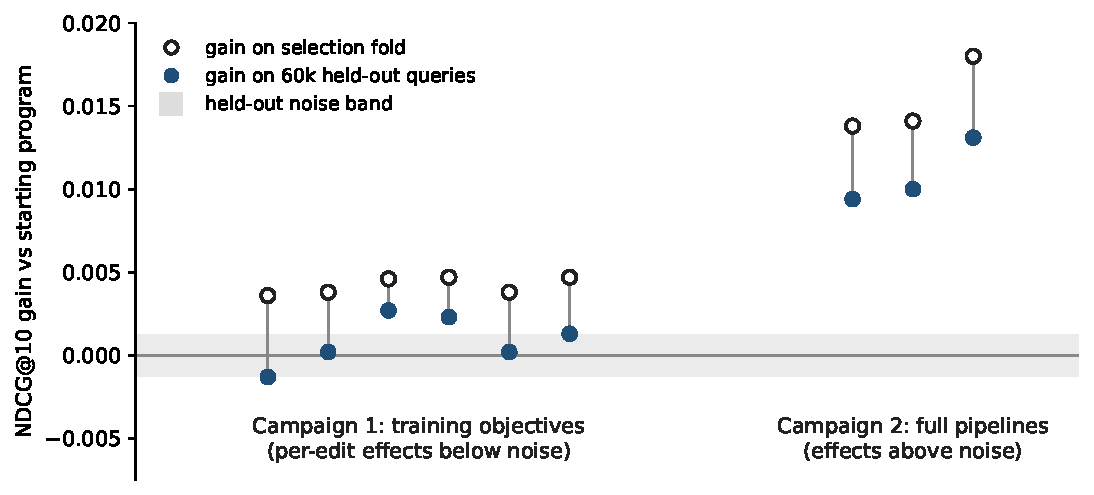
\includegraphics[width=\linewidth]{transfer_contrast.pdf}
{\SmallSize Per-run NDCG@10 gains over the starting program, on the selection
fold (open) vs 60k held-out queries (filled). Campaign 1 collapses into the
noise band; campaign 2 survives.}\\[8mm]

{\SmallSize \textbf{Open everything}: code, configs, seeds, logs, discovered
programs, audit scripts at {\ttfamily github.com/shabazpatel/evorank}.
Limitations: one dataset (the only public LTR set with conversion and
revenue labels); three runs per condition; revenue is a proxy; audited for
transfer, not online effects.}
\end{minipage}

\vfill
\begin{tcolorbox}[enhanced,colback=goldfill,colframe=goldedge,boxrule=1.5pt,
  arc=4mm,left=10mm,right=10mm,top=6mm,bottom=6mm]
{\fontsize{42}{48}\selectfont\bfseries\color{goldedge}Use this on your ranking stack}\\[4mm]
\newcommand{\Step}[2]{\begin{minipage}[t]{0.188\textwidth}
{\BodySize\bfseries\color{goldedge}#1}\\[2mm]{\SmallSize #2}\end{minipage}}
\Step{1. Measure noise}{Paired query bootstrap on the evaluation fold you
can afford: that half-width is your noise floor.}\hfill
\Step{2. Hand-build one candidate}{One reference candidate from your
domain's literature, before any LLM spend.}\hfill
\Step{3. Gate the space}{Require its gain $\ge 2.5\times$ the noise floor.
No headroom, no loop: keep your budget.}\hfill
\Step{4. Run guarded}{Leakage-safe statistics, whitelists, budgets, and
rejection messages the model learns from.}\hfill
\Step{5. Audit, then believe}{A held-out transfer audit, never the loop's
own scores, decides what counts.}
\end{tcolorbox}
\vspace{5mm}
{\color{accent}\rule{\textwidth}{1.5pt}}\\[3mm]
{\FootSize\textbf{Contact:} rayhanbp@umd.edu \,\textbullet\, shabaz.b.patel@gmail.com
\hfill Paper + proceedings: genai-ecommerce.github.io/GenAIECommerce2026}
\end{document}
